\section{Square Ice Shelf}
This is an example of velocity computation in steady state for a square ice shelf. First, launch MATLAB. In the left sidebar, select \verb@ISSM_DIR@ (the directory in which ISSM is stored) as your Current Directory. Then, navigate to \verb@examples/SquareIceshelf@, which you can also do via the left sidebar or by running the following in the MATLAB Command Window:
\begin{verbatim}>> cd examples/SquareIceShelf\end{verbatim}

You can create an empty model structure by running:
\begin{verbatim}>> md=model;\end{verbatim}

Create a mesh of the domain outline with a resolution of 50,000 meters:
\begin{verbatim}>> md=triangle(md,'DomainOutline.exp',50000);\end{verbatim}

Define the glacier system as an ice shelf (no island):
\begin{verbatim}>> md=setmask(md,'all','');\end{verbatim}

Parameterize the model with the file \verb@Square.par@ (which you can see exists in the current directory by inspecting the left sidebar):
\begin{verbatim}>> md=parameterize(md,'Square.par');\end{verbatim}

Define all elements as SSA:
\begin{verbatim}>> md=setflowequation(md,'SSA','all');\end{verbatim}

Compute the velocity field of the ice shelf:
\begin{verbatim}>> md=solve(md,'Stressbalance');\end{verbatim}

Finally, generate a plot of the velocity:
\begin{verbatim}>> plotmodel(md,'data',md.results.StressbalanceSolution.Vel);\end{verbatim}

\begin{figure}[H]
	\begin{center}
		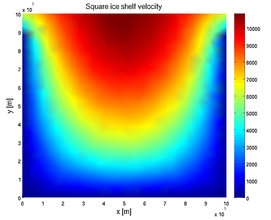
\includegraphics{/assets/img/tutorials/squareiceshelf/squarevel.png}
	\end{center}
\end{figure}
